% Rhizome neural operator: full model (top) and one synchronous update (bottom).
% Build: pdflatex rhizome_architecture.tex  ->  rhizome_architecture.pdf
% Matches ebm21cm/model/rhizome.py and ebm21cm/model/recurrent.py (_RecurrentField2d).
\documentclass[tikz,border=3pt]{standalone}
\usepackage{amsmath,amssymb,bm}
\usetikzlibrary{arrows.meta,positioning,fit,backgrounds,calc}

% Okabe-Ito colours (colour-blind safe), same roles as in the animation
\definecolor{kern}{HTML}{0072B2}   % spatial interaction / kernel
\definecolor{srcg}{HTML}{D55E00}   % source gate B
\definecolor{recg}{HTML}{009E73}   % receiver gate A
\definecolor{pt}{HTML}{4D4D4D}     % pointwise operations

\tikzset{
  >={Latex[length=2.2mm,width=1.6mm]},
  every node/.style={font=\small},
  op/.style={draw=pt, rounded corners=2pt, fill=white, minimum height=8.5mm, inner xsep=5pt, align=center},
  var/.style={inner sep=2pt, align=center},
  sig/.style={op, fill=kern!10, draw=kern, line width=0.9pt},
  gate/.style={op, minimum width=9mm},
  dotop/.style={circle, draw=pt, fill=white, inner sep=0pt, minimum size=5.5mm, font=\normalsize},
  flow/.style={->, draw=pt, line width=0.6pt},
  aux/.style={->, draw=pt!60, line width=0.5pt},
  lbl/.style={font=\scriptsize, text=pt},
}

\begin{document}
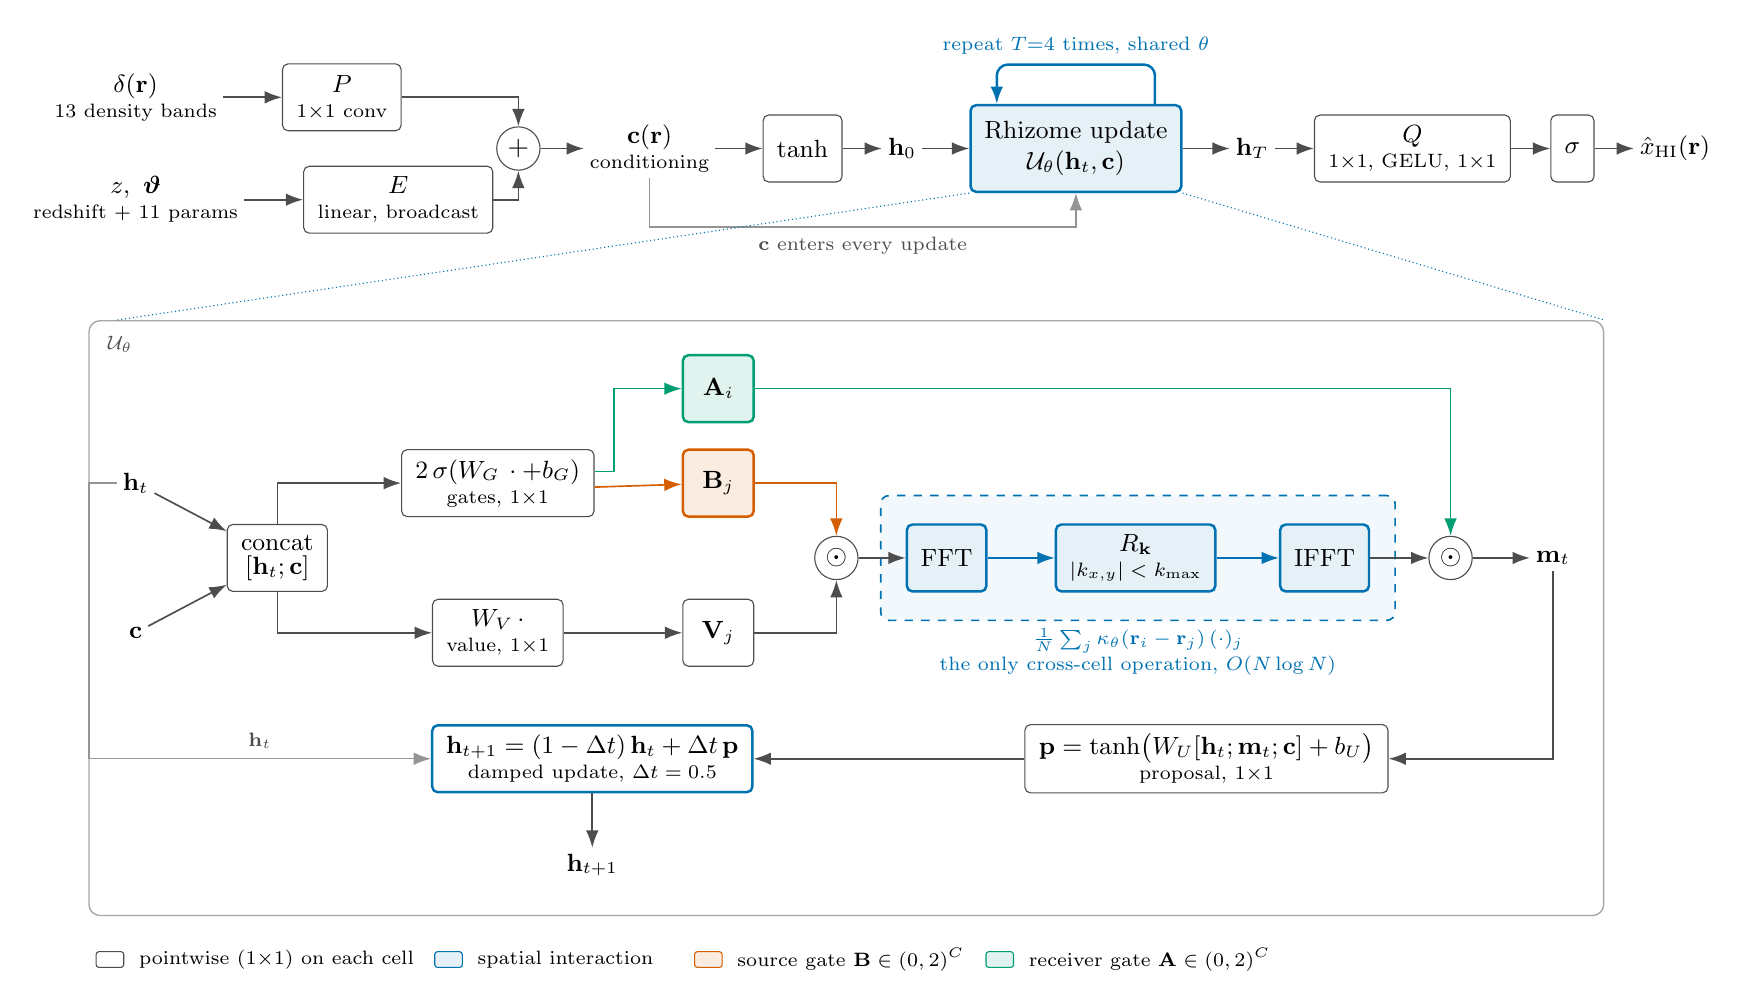
\begin{tikzpicture}

% ───────────── full model ─────────────
\node[var] (delta) at (0,0.55) {$\delta(\mathbf r)$\\[-2pt]{\scriptsize 13 density bands}};
\node[var] (scal) at (0,-0.75) {$z,\ \bm\vartheta$\\[-2pt]{\scriptsize redshift + 11 params}};
\node[op, right=0.75 of delta] (lift) {$P$\\[-2pt]{\scriptsize $1{\times}1$ conv}};
\node[op, right=0.75 of scal] (emb) {$E$\\[-2pt]{\scriptsize linear, broadcast}};
\node[dotop] (plus) at ($(lift.east)!0.5!(emb.east)+(0.9,0)$) {$+$};
\node[var, right=0.55 of plus] (c) {$\mathbf c(\mathbf r)$\\[-2pt]{\scriptsize conditioning}};
\node[op, right=0.6 of c] (tanh0) {$\tanh$};
\node[var, right=0.5 of tanh0] (h0) {$\mathbf h_0$};
\node[sig, right=0.6 of h0, minimum width=24mm, minimum height=11mm] (U) {Rhizome update\\$\mathcal U_\theta(\mathbf h_t,\mathbf c)$};
\node[var, right=0.6 of U] (hT) {$\mathbf h_T$};
\node[op, right=0.5 of hT] (Q) {$Q$\\[-2pt]{\scriptsize $1{\times}1$, GELU, $1{\times}1$}};
\node[op, right=0.5 of Q] (sg) {$\sigma$};
\node[var, right=0.5 of sg] (out) {$\hat x_{\mathrm{HI}}(\mathbf r)$};

\draw[flow] (delta) -- (lift);
\draw[flow] (scal) -- (emb);
\draw[flow] (lift.east) -| (plus.north);
\draw[flow] (emb.east) -| (plus.south);
\draw[flow] (plus) -- (c);
\draw[flow] (c) -- (tanh0);
\draw[flow] (tanh0) -- (h0);
\draw[flow] (h0) -- (U);
\draw[flow] (U) -- (hT);
\draw[flow] (hT) -- (Q);
\draw[flow] (Q) -- (sg);
\draw[flow] (sg) -- (out);
% conditioning re-enters every update
\draw[aux] (c.south) -- ++(0,-0.62) -| node[lbl, pos=0.25, below] {$\mathbf c$ enters every update} (U.south);
% recurrence loop with shared weights
\draw[->, draw=kern, line width=0.9pt, rounded corners=4pt] ($(U.north east)+(-0.35,0)$) -- ++(0,0.5)
  -- node[lbl, above, text=kern] {repeat $T{=}4$ times, shared $\theta$} ($(U.north west)+(0.35,0.5)$) -- ($(U.north west)+(0.35,0)$);

% ───────────── one update ─────────────
\begin{scope}[yshift=-4.6cm]
\node[var] (ht) at (0,0.25) {$\mathbf h_t$};
\node[var] (cc) at (0,-1.65) {$\mathbf c$};
\node[op] (cat) at (1.8,-0.7) {concat\\[-2pt]$[\mathbf h_t;\mathbf c]$};
\node[op] (G) at (4.6,0.25) {$2\,\sigma(W_G\,\cdot+b_G)$\\[-2pt]{\scriptsize gates, $1{\times}1$}};
\node[op] (V) at (4.6,-1.65) {$W_V\,\cdot$\\[-2pt]{\scriptsize value, $1{\times}1$}};
\node[gate, draw=recg, fill=recg!12, line width=0.9pt] (A) at (7.4,1.45) {$\mathbf A_i$};
\node[gate, draw=srcg, fill=srcg!12, line width=0.9pt] (B) at (7.4,0.25) {$\mathbf B_j$};
\node[gate, fill=white] (Vj) at (7.4,-1.65) {$\mathbf V_j$};
\node[dotop] (m1) at (8.9,-0.7) {$\odot$};
\node[sig] (fft) at (10.3,-0.7) {FFT};
\node[sig] (R) at (12.7,-0.7) {$R_{\mathbf k}$\\[-2pt]{\scriptsize $|k_{x,y}|<k_{\max}$}};
\node[sig] (ifft) at (15.1,-0.7) {IFFT};
\node[dotop] (m2) at (16.7,-0.7) {$\odot$};
\node[var] (m) at (18.0,-0.7) {$\mathbf m_t$};
\node[op] (prop) at (13.6,-3.25) {$\mathbf p=\tanh\!\big(W_U[\mathbf h_t;\mathbf m_t;\mathbf c]+b_U\big)$\\[-2pt]{\scriptsize proposal, $1{\times}1$}};
\node[op, draw=kern, line width=0.9pt] (upd) at (5.8,-3.25) {$\mathbf h_{t+1}=(1-\Delta t)\,\mathbf h_t+\Delta t\,\mathbf p$\\[-2pt]{\scriptsize damped update, $\Delta t=0.5$}};
\node[var] (hn) at (5.8,-4.6) {$\mathbf h_{t+1}$};

\draw[flow] (ht) -- (cat);
\draw[flow] (cc) -- (cat);
\draw[flow] (cat) |- (G);
\draw[flow] (cat) |- (V);
\draw[flow, draw=recg] (G.east) ++(0,0.15) -- ++(0.25,0) |- (A);
\draw[flow, draw=srcg] (G.east) ++(0,-0.05) -- (B);
\draw[flow] (V) -- (Vj);
\draw[flow, draw=srcg] (B.east) -| (m1.north);
\draw[flow] (Vj.east) -| (m1.south);
\draw[flow] (m1) -- (fft);
\draw[flow, draw=kern] (fft) -- (R);
\draw[flow, draw=kern] (R) -- (ifft);
\draw[flow] (ifft) -- (m2);
\draw[flow, draw=recg] (A.east) -| (m2.north);
\draw[flow] (m2) -- (m);
\draw[flow] (m.south) |- (prop.east);
\draw[flow] (prop) -- (upd);
\draw[flow] (upd) -- (hn);
\draw[aux] (ht.west) -- ++(-0.35,0) |- (upd.west) node[lbl, pos=0.75, above] {$\mathbf h_t$};

\begin{scope}[on background layer]
  \node[fit=(fft)(R)(ifft), inner xsep=9pt, inner ysep=10pt, rounded corners=3pt,
        fill=kern!5, draw=kern, dashed, line width=0.6pt,
        label={[lbl, text=kern, yshift=1pt, align=center]below:{$\tfrac1N\sum_j \kappa_\theta(\mathbf r_i-\mathbf r_j)\,(\cdot)_j$\\the only cross-cell operation, $O(N\log N)$}}] (spec) {};
  \node[fit=(ht)(cc)(A)(m)(prop)(upd)(hn)(spec), inner xsep=10pt, inner ysep=12pt, rounded corners=4pt,
        draw=pt!50, line width=0.5pt] (panel) {};
\end{scope}
\node[lbl, anchor=north west, font=\scriptsize\bfseries] at ($(panel.north west)+(0.12,-0.08)$) {$\mathcal U_\theta$};
\end{scope}

% zoom connectors
\draw[densely dotted, draw=kern] (U.south west) -- (panel.north west -| ht.west);
\draw[densely dotted, draw=kern] (U.south east) -- (panel.north east);

% legend
\begin{scope}[shift={($(panel.south west)+(0.1,-0.55)$)}, every node/.style={font=\scriptsize, anchor=west}]
  \draw[draw=pt, fill=white, rounded corners=1pt] (0,-0.1) rectangle (0.35,0.1); \node at (0.42,0) {pointwise ($1{\times}1$) on each cell};
  \draw[draw=kern, fill=kern!10, rounded corners=1pt] (4.3,-0.1) rectangle (4.65,0.1); \node at (4.72,0) {spatial interaction};
  \draw[draw=srcg, fill=srcg!12, rounded corners=1pt] (7.6,-0.1) rectangle (7.95,0.1); \node at (8.02,0) {source gate $\mathbf B\in(0,2)^{C}$};
  \draw[draw=recg, fill=recg!12, rounded corners=1pt] (11.3,-0.1) rectangle (11.65,0.1); \node at (11.72,0) {receiver gate $\mathbf A\in(0,2)^{C}$};
\end{scope}

\end{tikzpicture}
\end{document}
